% Suppress some compilation warnings
\RequirePackage[save,showerrors]{silence}
\WarningFilter{biblatex}
  {The starred command '\DeclareDelimAlias*' is} % APA package is using this deprecated starred version
\WarningFilter{transparent}
  {Loading aborted} % Used by the svg package

\documentclass[usenames,dvipsnames,10pt]{beamer}

% languages typesetting rules
\usepackage[main=french,english]{babel}

% links configuration
\usepackage{hyperref} % commands such as \href, \url, etc.
\hypersetup{
    colorlinks=true,
    linkcolor=,
    urlcolor=NavyBlue,
    citecolor=Green
}

% bibliography configuration
\usepackage[style=apa,backref=true]{biblatex}

\usepackage{csquotes} % biblatex extensions for non-english languages
\usepackage{caption} % more control over captions
\usepackage{subcaption} % for subfigures
\usepackage{ccicons} % icons for Creative-Commons licenses
\usepackage{hologo} % tex and co. logos
\usepackage[inkscapepath=./build/svg-inkscape/]{svg}

\graphicspath{{images/} {../images}}

% Beamer theme configuration
\usetheme{metropolis}
\metroset{sectionpage=progressbar, progressbar=frametitle}
\setbeamertemplate{caption}[numbered] % Show figure number when using `\caption` instead of `\caption*`
\setbeamertemplate{footline}[page number] % Show the current page number in the bottom line of each slide
% \setbeameroption{show only notes}

% Bibliography configuration
\bibliography{../references.bib}

% Meta information about this presentation
\title{L'identification des projets de logiciel libre accessibles aux nouveaux contributeurs}
\subtitle{Mémoire de Master Sciences de l'Éducation, parcours SYNVA}
\titlegraphic{
\includegraphics[width=0.25\textwidth]{unistra}}
\institute[]{\href{https://creativecommons.org/licenses/by-sa/4.0/}{\ccbysa}}
\author[PH]{Paul Hervot}
\date{8 septembre 2022}

\begin{document}

\frame{\titlepage{}}

\section{Évolution du sujet}

\begin{frame}[fragile]{Parcours personnel}
    \begin{figure}
        
\includegraphics[width=0.36\textwidth]{epita}
        
\includegraphics[width=0.27\textwidth]{prologin}
        
\includegraphics[width=0.27\textwidth]{fosdem}
    \end{figure}

    \note[item]{Parcours perso informatique + éducation avec EPITA}
    \note[item]{Attrait logiciel libre avec Prologin et les rendez-vous au
    FOSDEM}
\end{frame}

\begin{frame}[fragile]{Idée de départ}
    Axe enseignement et logiciel libre.

    Approche initiale enseignement $\rightarrow$ recherche de cours existants.

    Faire une étude de besoin ?

    Évaluer le succès d'une formation existante ?
\end{frame}

\begin{frame}{Littérature sur les barrières d'entrée}
    Beaucoup d'articles de Igor Steinmacher.

    Recherche principalement qualitative grandissante et très intéressante.

    Début de recherche quantitative, notamment avec \textcite{signals-2019}.

    \note[item]{%
        Steinmacher est partout et utilise des méthodologies qualitatives très
        intéressantes, c'est rigolo mais donc j'ai voulu trouver d'autres
        auteurs et d'autres approches sur le sujet
    }
    \note[item]{%
        Très dur de naviguer la littérature, mon approche était de chercher des
        mots-clés puis d'approfondir en suivant les études citées par les
        articles que je trouvais.
    }
    \note[item]{%
        Une approche quantitative avec minage de projets me permettrait d'être
        d'exploiter un peu plus mes compétences existantes afin de me concentrer
        sur certains aspects recherche.
    }
\end{frame}

\section{L'archive de Software Heritage}

\begin{frame}[fragile]{Idée venant de mes relations}
    \begin{figure}
        \includesvg[width=0.5\textwidth]{softwareheritage}
    \end{figure}

    Connu via la thèse d'un ami : \emph{\citetitle{swh-seirl}},
    \textcite{swh-seirl}.

    Permet de construire à partir de \textcite{signals-2019}.

    \note[item]{%
        Approche suffisamment nouvelle pour que je puisse apprendre des choses
        sur la collecte de donnée, tout en se basant sur certaines technologies
        que je connais, donc moins perdre de temps sur des questions purement
        techniques
    }
\end{frame}

\begin{frame}{Formateur, même techniquement}
    Java et big data.

    Accès temporaire au serveur, travail sous contrainte de temps $\rightarrow$
    plusieurs solutions de secours.

    Trois jours d'exécution (malgré une forte parallélisation).
\end{frame}

\section{L'analyse statistique sans distribution normale}

\begin{frame}{Outils utilisés}
    Les classiques : numpy, scipy, matplotlib.

    Plus spécialisé : pandas (similarités avec le R), statsmodels.

    \note[item]{%
        J'ai essayé de rendre le code le plus lisible et réutilisable possible,
        mentionner aussi le replication package ?
    }
\end{frame}

\begin{frame}{Traitement de la présence d'instructions de contribution}
    \begin{figure}
        \begin{subfigure}[t]{0.45\textwidth}
            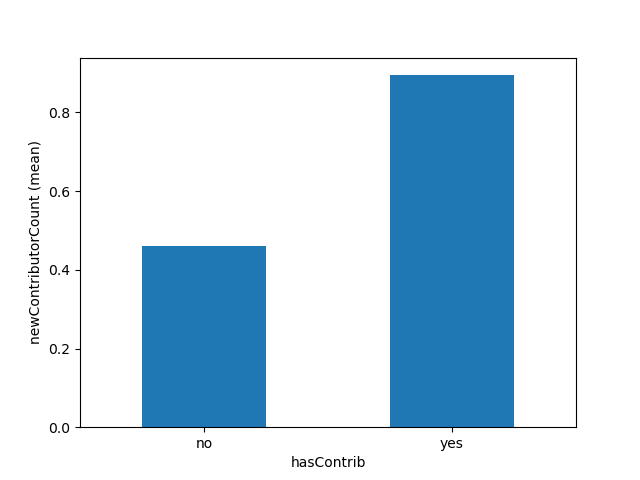
\includegraphics[width=\textwidth]{../experiment/data_analysis/hasContrib_meanNewContributorCount.png}
            \caption{Moyenne du nombre de nouveaux contributeurs pour chaque catégorie}
        \end{subfigure}
        \begin{subfigure}[t]{0.45\textwidth}
            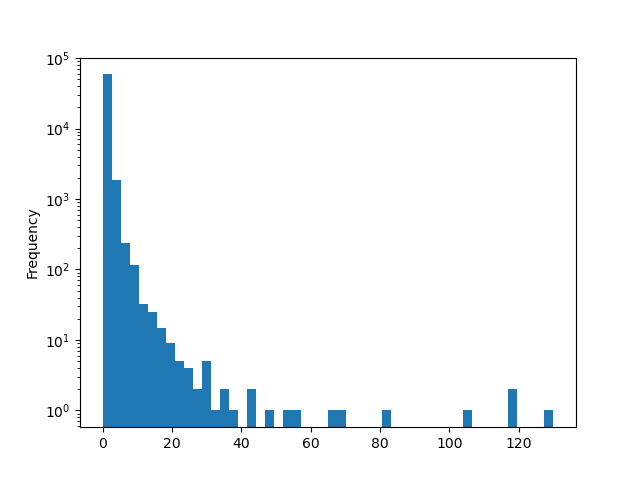
\includegraphics[width=\textwidth]{../experiment/data_analysis/newContributorCount_distribution.png}
            \caption{Nombre de nouveaux contributeurs\\(ordonnées logarithmiques)}
        \end{subfigure}
    \end{figure}

    Vu en cours : test de Fisher et test de Student $\rightarrow$ paramétriques

    Non paramétrique : test de Wilcoxon-Mann-Whitney.
\end{frame}

\section{Bibliographie}

\begin{frame}[allowframebreaks]{Bibliographie}
    \printbibliography{}
\end{frame}

\end{document}
